% !TeX spellcheck = cs_CZ
%{\tikzset{external/prefix={tikz/FYZI/}}
% \tikzset{external/figure name/.add={ch43_}{}}
%=========================== Kapitola: Difuze =====================================================
\setchaptertoc
\chapter{Difuze}\label{fyz:IchapXLIII}

  \section{Srážky molekul}\label{fyz:IchapXLIIIsecI}
  \section{Střední volná dráha}\label{fyz:IchapXLIIIsecII}
  \section{Driftová rychlost}\label{fyz:IchapXLIIIsecIII}
  \section{Iontová vodivost}\label{fyz:IchapXLIIIsecIV}
  \section{Molekulová difuze}\label{fyz:IchapXLIIIsecV}
  \section{Tepelná vodivost}\label{fyz:IchapXLIIIsecVI}
  \section{Příklady a cvičení}\label{fyz:IchapXLIIIsecVII}

  \begin{figure}[hb!] %\ref{fyz:fig0478}
    \centering
    \subcaptionbox{\label{fyz:fig0478a}}{\luafigure[0.4]{fyz_fig0478a.pdf}}  \\
    \subcaptionbox{\label{fyz:fig0478b}}{\luafigure[0.6]{fyz_fig0478b.pdf}}  
    \caption{
             (\cite[s.~601]{Feynman01}).}
    \label{fyz:fig0478}
  \end{figure}

    \begin{figure}[ht!] %\ref{fyz:fig0479}
      \centering
      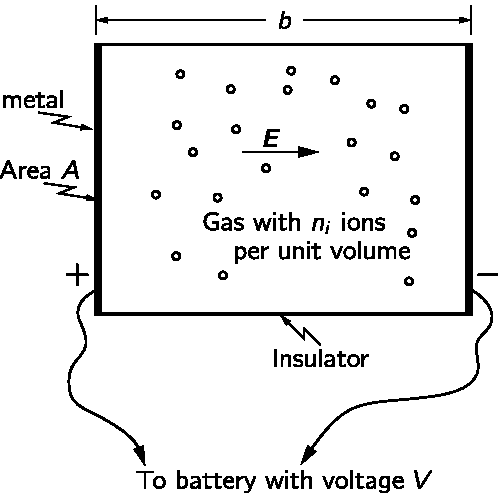
\includegraphics[width=0.7\linewidth]{fyz_fig0479.pdf}
      \caption{ 
               (\cite[s.~707]{Feynman01})}
      \label{fyz:fig0479}
    \end{figure}
    \todo[inline]{Kapitola fey1ch43 je zcela prázdná, pouze obrázky}   
%} %tikzset
%---------------------------------------------------------------------------------------------------